\section{Dokumentengeschichte}
\begin{table}[h]
 \begin{tabular}{|l|l|p{4cm}|}
 \hline
 Zeitraum & PL/Autor(en) & Änderungen \\
 \hline
 Wintersemester 2017/18 & Behzad Karimi & 
Erste Version des Textes eingefügt\newline 
text \newline 
text \newline 
text \newline 
text \newline 
text \newline 
 
  \\
 \hline
 \end{tabular}
 \caption{Dokumentengeschichte}
 \end{table}

\section{Aufgabe der Komponente}
\begin{figure}[h!]
\centering
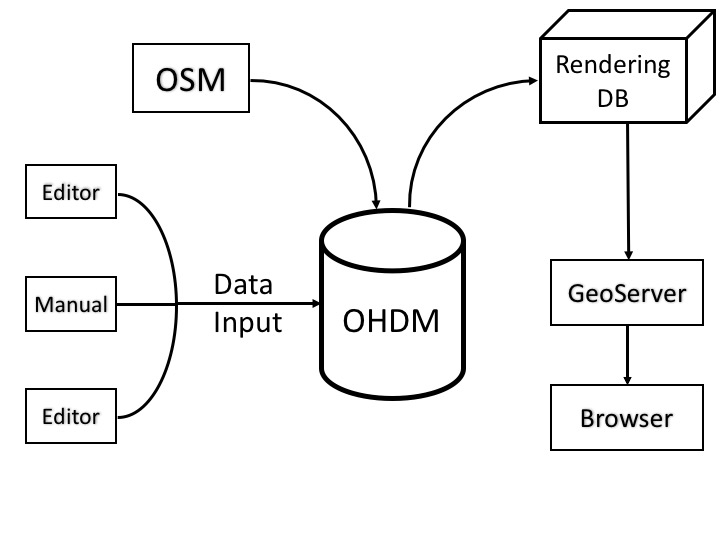
\includegraphics[page=1, width=127mm]{ohdm_datenmodell/Bilder/data.jpg}
\caption{OHDM Datamodell}
\label{fig:datamodell}
\end{figure}
%TODO Text zum Bild :)

\begin{figure}[h!]
\centering
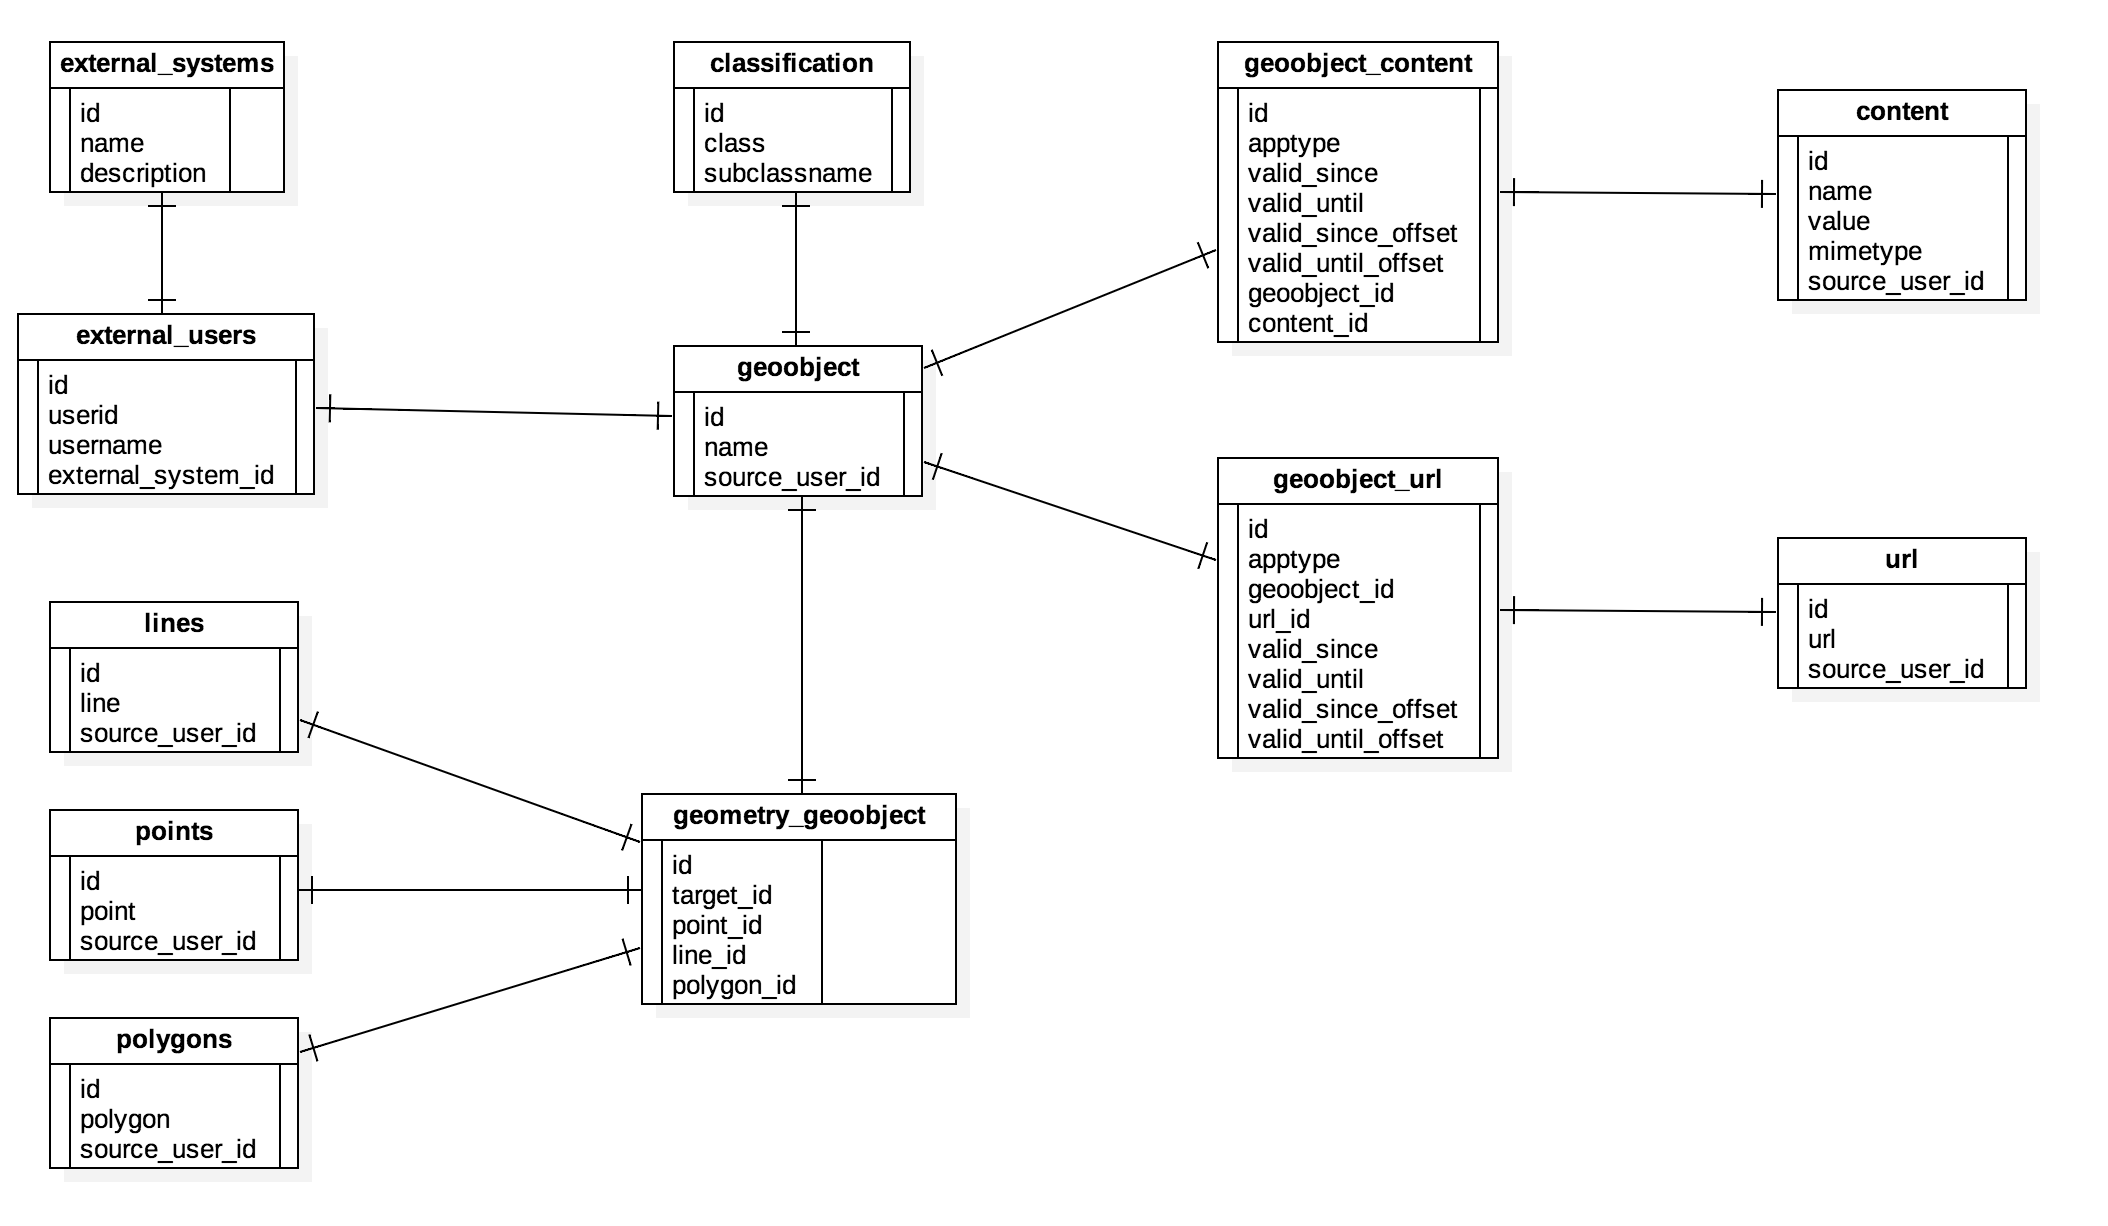
\includegraphics[width=127mm]{ohdm_datenmodell/Bilder/ohdm_data_modell.png}
\caption{OHDM Datamodell}
\label{fig:datamodell}
\end{figure}
Im Datenmodell von OHDM geht alles vom Geoobjekt (geoobject) aus. Dieses zentrale Object beschreibt alle Modelle auf der Karte, da alle Informationen der Modelle auf das geobject verweisen. Das einzige Objekt worauf das geobject verweist, ist der Ersteller (external\_users). Der Ersteller des Objekts greift durch ein externes System (external\_systems) auf dern Server zu und gibt die Informationen über das Geobjekt weiter. Wie nun ein Geobjekt im Allgemeinen aussieht wird im nächsten Abschnitt beschrieben.

\subsection{Geometrien in GIS}
Da OHDM mit PostGIS arbeitet (für GIS siehe ...) werden die zweidimensionalen Objekte als Polygone repräsentiert. Polygone bestehen dabei aus Punkten (points) und Linien (lines). Die Punkte werden mit Linien verbunden, so dass am Ende ein Polygon entsteht. Der folgende Satz ist dabei eine Vorraussetzung für einen Polygon:
\begin{center}
 \textit{Ein Polygon, eine geoordete Menge von Strecken, mit der Eigenschaft, dass ein Punkt der letzten Strecke identisch zu einem Punkt der ersten Strecke ist.}
 \end{center} 
Das heißt ein Polygon kann ohne Punkte und Linien nicht existieren. Ebenso kann eine Linie ohne zwei Punkte nicht existieren. Wie erstellt man nun ein Gebäudekomplex aus mehreren Gebäuden? Diese sogenannten \textit{Multi-Polygone}, sind mehrere nicht überlappende Polygone. Dann gibt es noch die Möglichkeit Löcher in den Polygonen zu erstellen. Diese Löcher sind nichts weiter als ein Polygon in einem anderen Polygon. In GIS gibt es dabei folgende Einschränkungen:
\begin{itemize}
\item Polygone im inneren dürfen sich untereinander nicht überlappen. Falls doch, könnten sie auch als ein einzelnes Polygon dargestellt werden.
\item Ein Rand eines inneren Polygons darf nicht Rand des äußeren Polygons sein. Falls dem nämlich so ist, wird das äußere Polygon nämlich anders dargestellt werden.
\item Aus dem oberen Satz lässti sich auch folgende Eigenschaft erklären. Kein Punkt des inneren Polygons darf gleichzeitig dem äußerem Polygon gehören. Hier würden ebenfalls das äußere Polygon ansonsten anders dargestellt werden. 
\end{itemize}
%TODO  Rendering
Wie genau nun Objekte enstehen und Polygone dargestellt werden, wird im Kapitel ( Diehe Kapitel Rendering) genauer erläutert. Damit die Polygone bzw. Geobjekte ordentlich auf der Karte dargestellt werden können, teilem wir jedem Geoobjekt eine Klasse (class) zu. 

\subsection{Klassifikation von Geoobjekten}
Die Entity classification weißt mit einer ID auf das Geoobjekt hin und teilt diesen in eine bestimmte Klasse ein. Jede Klasse hat wiederum nochmals Unterklassen. Dadurch können wir Geoobjekte genau beschreiben um diese auf der Karte dementsprechend anzuzeigen. Die genaue Einteilung der Klassen und Unterklassen kann man in den Datenbank Tabellen ablesen oder auf der Wiki Seite von \href{http://wiki.openstreetmap.org/wiki/Map_Features#Building}{OSM} finden. 
Nun können wir Geoobjekte darstellen und erklären zu welcher Klasse bzw. Unterklasse diese gehören. Wie nun genau ein Polygon dargestellt wird und welche Informationen angezeigt werden, erklären wir im nächsten Abschnitt.

\subsection{Informationen eines Geoobjekts}
Die Informationen über ein Geoobjekt werden in den Instanzen geoobject\_content und content beschrieben. Dazu gehören auch die zeitlichen Informationen, die beschreiben, in welchem Zeitraum das Objekt existierte bzw. seit wann es existiert.  \\
In der Instanz geobject\_url wird eine URL gespeichert die auf eine Webseite des Objektes verweist. Dies kann z.B. die Homepage, Wikipedia Eintrag, etc. sein. Dazu gibt es noch die Instanz url, hier können zusätzliche Links gespeichert werden mit weiteren Informationen über das jeweilige Geobjekt.s

%TODO Webschnittstelle die die Editoren untersützt, Webschnittstelle für den Import

\section{Architektur}

\subsection{Überlick}
Grafik der Teile der Komponente (wichtig: Benennung aller Schnittstellen). 
Anwendung der Komponente nennen (Use Case).

Übliche Interaktionen durch Interaktionsdiagramme.

(Ausfüllen in Prototyp-Phase)

\subsection{Schnittstellendefinitionen}
Beschreibung der angebotenen Schnittstellen. Benennung der Funktionen
mit Vor- und Nachbedingungen. Beschreibuung des Protocol-Bindings.

(Beginnen in Prototyp-Phase. Konkretisieren in der Alphaphase)

\subsection{genutztes Komponenten}
Beschreibung, welche weiteren Komponenten (in welchen Versionen, wo beziehbar) genutzt werden.

(Beginnen in Prototyp-Phase. Konkretisieren in der Alphaphase)

\section{Nutzung}
\subsection{Code}
Wo findet man den Code. Struktur des Codes. (In Prototyphase ausfüllen,
kann dort sehr kurz sein. Ab Alpha-Phase konkret beschreiben.)

\subsection{Deployment / Runtime}
Beschreibung wie die Komponenten aus dem Quellcode erzeugt werden kann,
wie sie installiert wird und wie man sie startet.

\section{Qualitätssicherung}
(Ausfüllen ab Alpha-Phase).

Wie erfolgt die Sicherung der Qualität? Keine Romane, sondern ehrlich notieren,
was man tut. Wenn man nichts tut, dann steht hier: Wir sichern die Qualität der
Komponente nicht.

Issue-Tracking: wie erfolgt das, interne Fehlermeldungen (ab Alpha), 
externe Fehlermeldungen ab Beta.

\subsection{Test}
Wie wird die Komponente getestet.

\section{Vorschläge / Ausblick}
Was ist aufgefallen, was sollte man ändern? Löschen Sie auch gern die Kommentare
der Vorgänger, aber nur, wenn es wirklich nicht mehr relevant ist.